%
% $RCSfile: loop_as_operation.tex,v $
%
% Copyright (C) 2002-2008. Christian Heller.
%
% Permission is granted to copy, distribute and/or modify this document
% under the terms of the GNU Free Documentation License, Version 1.1 or
% any later version published by the Free Software Foundation; with no
% Invariant Sections, with no Front-Cover Texts and with no Back-Cover
% Texts. A copy of the license is included in the section entitled
% "GNU Free Documentation License".
%
% http://www.cybop.net
% - Cybernetics Oriented Programming -
%
% http://www.resmedicinae.org
% - Information in Medicine -
%
% Version: $Revision: 1.1 $ $Date: 2008-08-19 20:41:07 $ $Author: christian $
% Authors: Christian Heller <christian.heller@tuxtax.de>
%

\subsubsection{Loop as Operation}
\label{loop_as_operation_heading}
\index{CYBOL Loop as Operation Example}

\emph{Looping} is a major technique for the effective processing of whole
stacks of data. As many other control structures, it is simplified to a logic
operation, in CYBOL.

\begin{figure}[ht]
    \begin{center}
        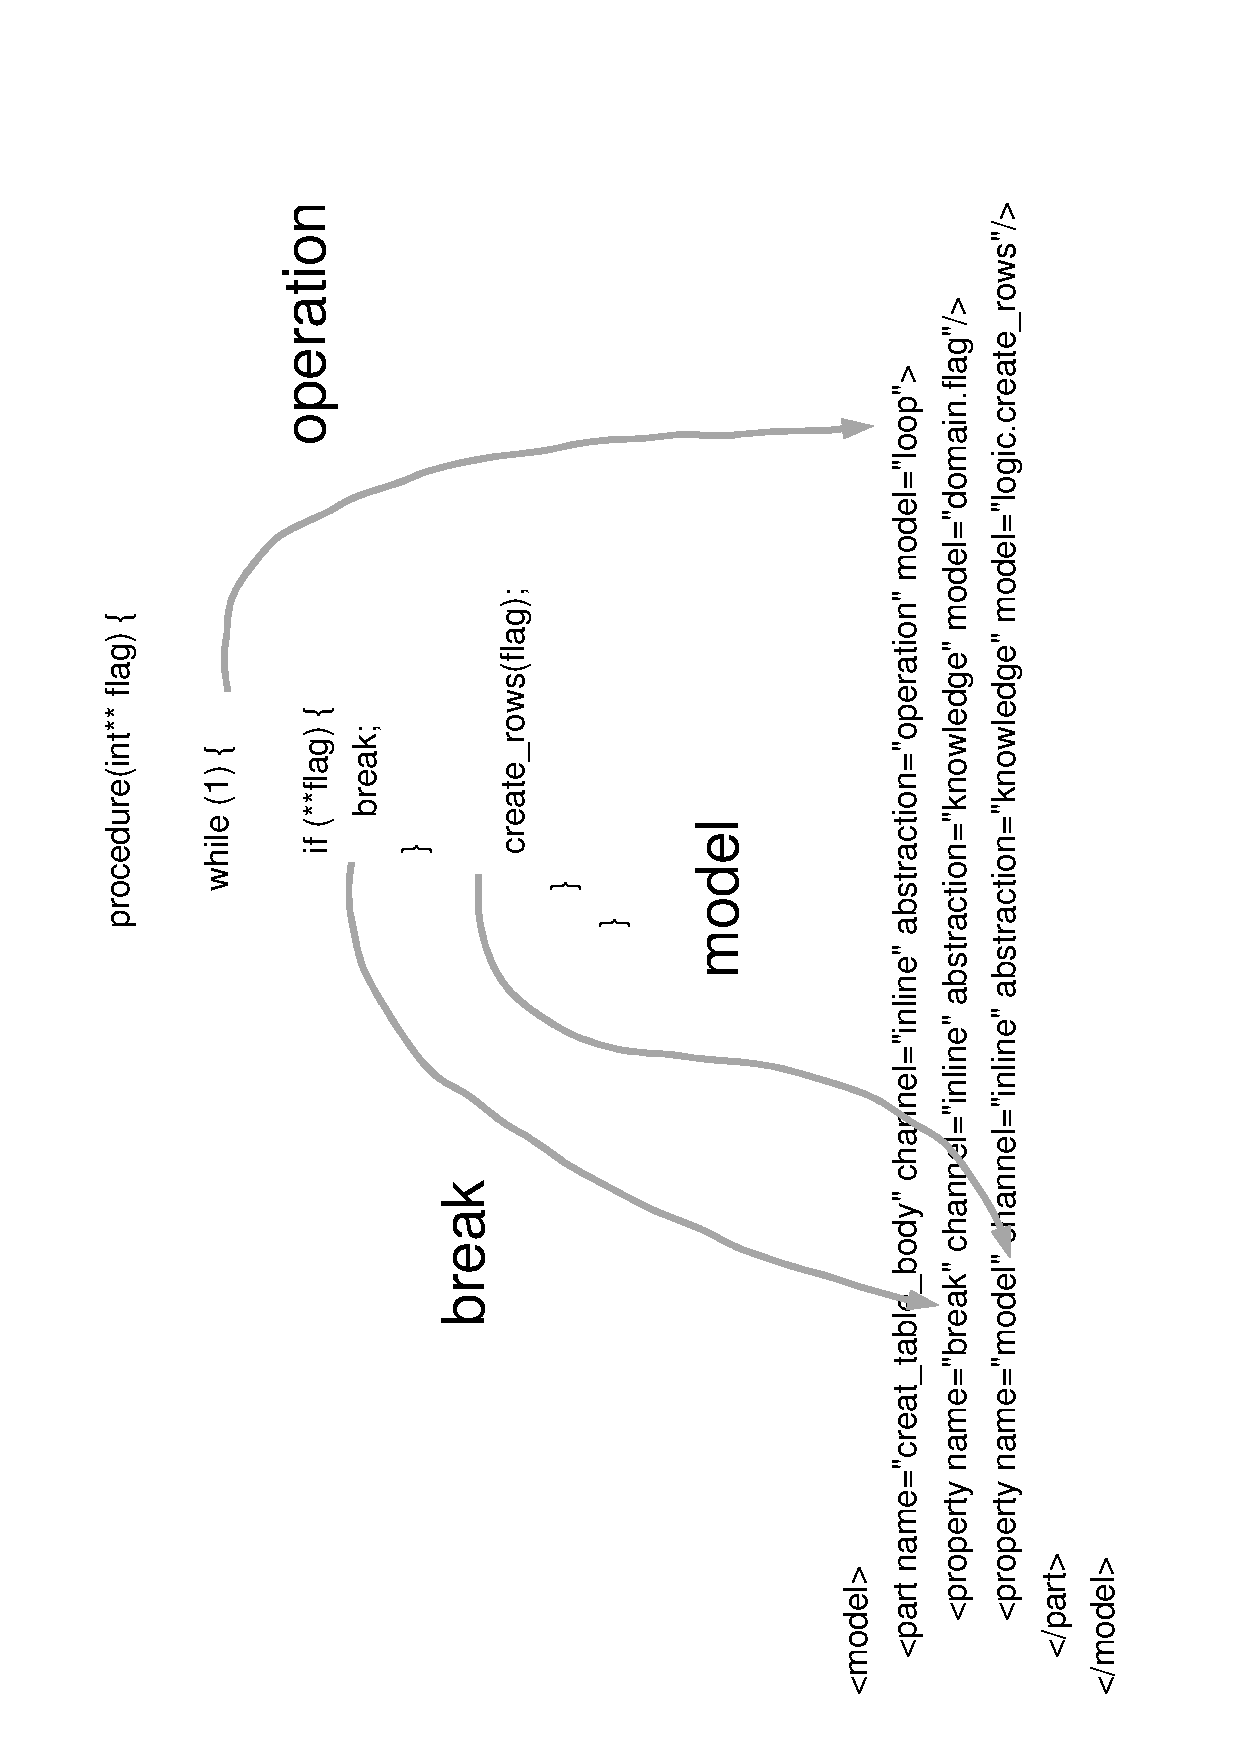
\includegraphics[scale=0.3,angle=-90]{graphic/cybolloop.pdf}
        \caption{Loop Control Structure and Elements in C and CYBOL}
        \label{cybolloop_figure}
    \end{center}
\end{figure}

The \emph{loop} operation needs two parameters to be functional: a \emph{break}
flag as means of interruption and a logic \emph{model} to be executed in each
loop cycle (figure \ref{cybolloop_figure}). An \emph{index} counting loop
cycles is not given, as it is in the responsibility of the logic \emph{model}
to manage that index, just like the setting of the \emph{break} flag,
internally. The following example dynamically creates a table consisting of a
number of rows:

\begin{scriptsize}
    \begin{verbatim}
<model>
    <part name="creat_table_body" channel="inline" abstraction="operation" model="loop">
        <property name="break" channel="inline" abstraction="knowledge" model="domain.flag"/>
        <property name="model" channel="inline" abstraction="knowledge" model="logic.create_rows"/>
    </part>
</model>
    \end{verbatim}
\end{scriptsize}
